\documentclass{article}
\usepackage[utf8]{inputenc}
\usepackage[hidelinks]{hyperref}

\title{Project Report}
\author{
    Nilabja Bhattacharya { Roll 2018201036}\\
  \texttt{nilabja.bhattacharya@students.iiit.ac.in}
  \and
    Praveen Balireddy {\ \ \  \ \ \ \ Roll 2018201052}\\
  \texttt{praveen.balireddy@students.iiit.ac.in}
}
\date{25th October 2018}
\usepackage{natbib}
\usepackage{graphicx}
\usepackage{longtable}

\begin{document}

\maketitle

\section{Objective}
Krukal’s algorithm implementation using vEB tree, Fibonacci heap and union find algorithm and their performance comparison

\section{Introduction}

\subsection{Minimum spanning tree}
A minimum spanning tree (MST) is a subset of the edges of a connected, weighted (un)directed graph that connects all the vertices together, without any cycles and with the minimum possible total edge weight. That is, it is a spanning tree whose sum of edge weights is as small as possible. More generally, any edge-weighted un-directed graph (not necessarily connected) has a minimum spanning forest, which is a union of the minimum spanning trees for its connected components.

\begin{figure}[h!]
\centering
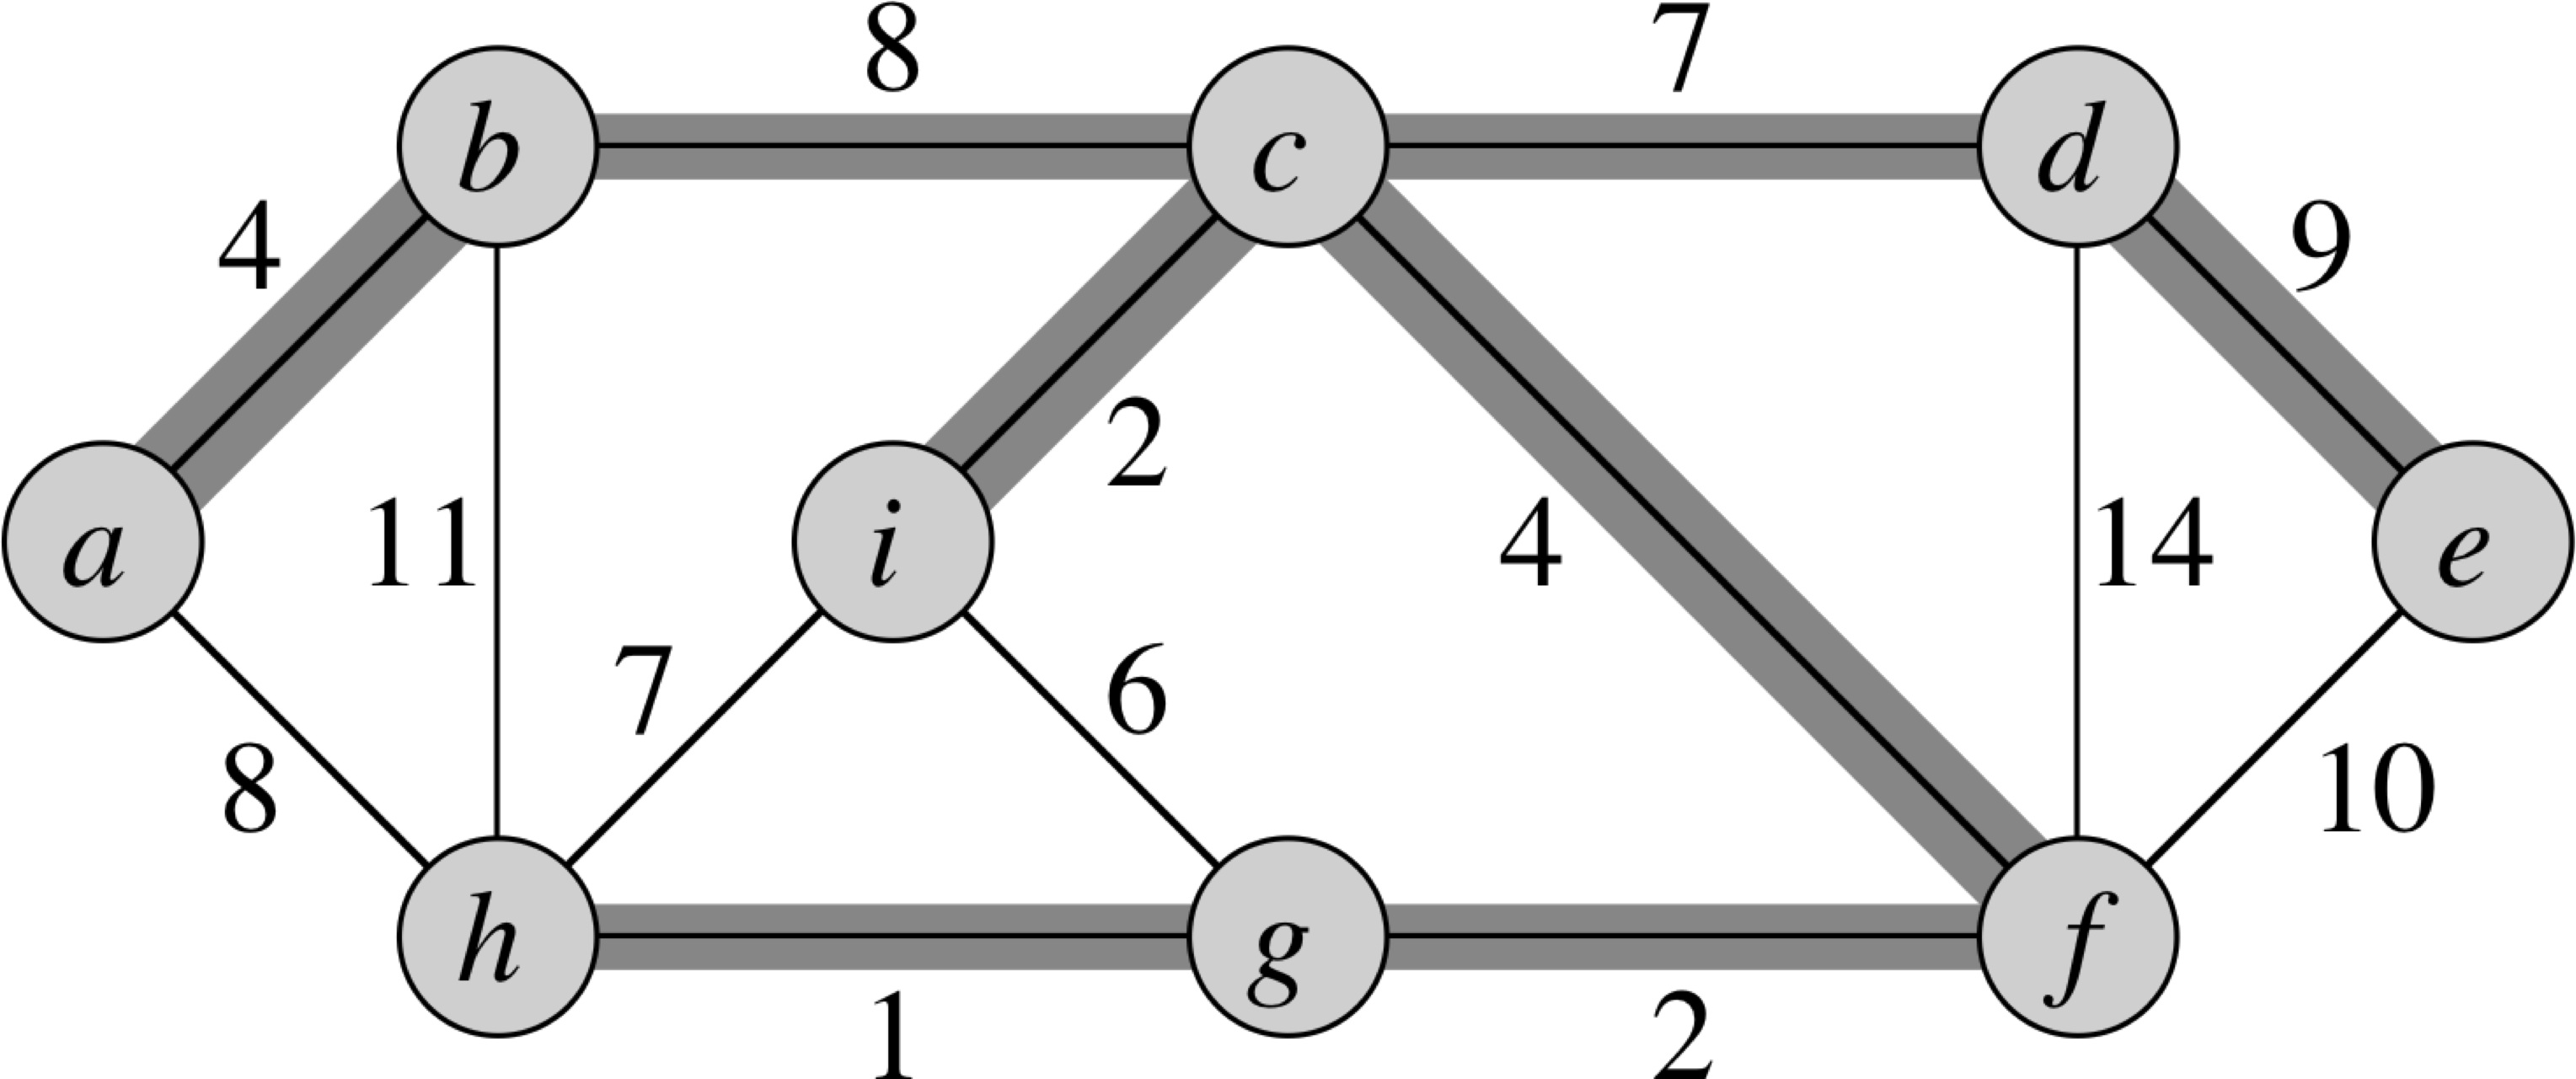
\includegraphics[width=0.7\columnwidth]{mst.jpg}
\caption{Minimum Spanning Tree}
\label{fig:MST}
\end{figure}


\subsubsection{Use cases}
\begin{enumerate}
\item Building a connected network: There are scenarios where we have a limited set of possible routes, and we want to select a subset that will make our network (e.g electrical grid, computer network) fully connected at the lowest cost
\item Clustering: If you want to cluster a bunch of points into k clusters, then one approach is to compute a minimum spanning tree and then drop the k-1 most expensive edges of the MST. This separates the MST into a forest with k connected components; each component is a cluster.
\end{enumerate}

\subsection{Kruskal Algorithm}
Kruskal's algorithm is a minimum-spanning-tree algorithm which finds an edge of the least possible weight that connects any two trees in the forest. It is a greedy algorithm in graph theory as it finds a minimum spanning tree for a connected weighted graph adding non decreasing cost edges at each step. This means it finds a subset of the edges that forms a tree that includes every vertex, where the total weight of all the edges in the tree is minimized. If the graph is not connected, then it finds a minimum spanning forest (a minimum spanning tree for each connected component). 

\subsection{Disjoint Data Structure}
A disjoint-set data structure is a data structure that tracks a set of elements partitioned into a number of disjoint (non-overlapping) subsets. It provides near-constant-time operations to add new sets, to merge existing sets, and to determine whether elements are in the same set. Disjoint-sets play a key role in Kruskal's algorithm for finding the minimum spanning tree of a graph.

\subsubsection{Operations}

\begin{enumerate}
    \item MakeSet: Makes a new set by creating a new element with a unique id, and initializing  the parent to itself. The MakeSet operation has O(1) time complexity, so initializing n sets has O(n) time complexity
    \item Find(x): Follows the chain of parent pointers from x till the root element, whose parent is itself. Returns the root element. Time Complexity: O(logn)
    \item Path compression: Path compression flattens the structure of the tree by making every node point to the root whenever Find is used on it. This is valid, since each element visited on the way to a root is part of the same set. The resulting flatter tree speeds up future operations not only on these elements, but also on those referencing them.
    \item Union(x,y): Merges x and y into the same partition by attaching the root of one to the root of the other. If this is done naively, such as by always making x a child of y, the height of the trees can grow as O(n). To prevent this union by rank or union by size is used by rank
\end{enumerate}
\paragraph{Union by rank:}Union by rank always attaches the shorter tree to the root of the taller tree. Thus, the resulting tree is no taller than the originals unless they were of equal height, in which case the resulting tree is taller by one node. In union by rank, each element is associated with a rank. Initially a set has one element and a rank of zero. If two sets are unioned and have the same rank, the resulting set's rank is one larger; otherwise, if two sets are unioned and have different ranks, the resulting set's rank is the larger of the two. Ranks are used instead of height or depth because path compression will change the trees' heights over time.
by size
\paragraph{Union by size:}In Union by size always attaches the tree with fewer elements to the root of the tree having more elements. 
With neither path compression (or a variant), union by rank, nor union by size, the height of trees can grow unchecked as O(n), which implies that Find and Union operations will take O(n) time.

\subsection{Fibonacci Heap}
A Fibonacci heap is a collection of rooted trees that are min-heap ordered. That is, each tree obeys the min-heap property : the key of a node is greater than or equal to the key of its parent. Figure 2 below shows an example of a Fibonacci heap. Each node x contains a pointer x.p to its parent and a pointer x.child to any one of its children. The children of x are linked together in a circular, doubly linked list, which we call the child list of x . Each child y in a child list has pointers y.left and y.right that point to y’s left and right siblings, respectively.  If node y is an only child, then y.left = y.right = y . Siblings may appear in a child list in any order.

\begin{figure}[h!]
\centering
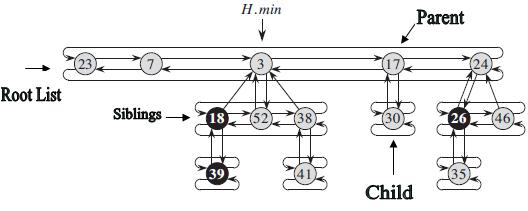
\includegraphics[width=0.9\columnwidth]{Fibbonaci.JPG}
\caption{Fibbonaci Heap}
\label{fig:fib1}
\end{figure}


\begin{enumerate}
\item Operation insert works by creating a new heap with one element and doing merge. Time Complexity: O(1)
\item Operation extract minimum operates in three phases. First we delete the root containing minimum element. It's children will become roots of new trees. If the number of children was d, it takes time O(d) to process all new roots. Time Complexity: O(d) = O(log n). 
\end{enumerate}

\subsection{vEB Tree}
A Van Emde Boas tree, also known as a vEB tree, is a tree data structure which stores integers between [0, n-1] for a positive integer n.  It performs all operations in O(log m) time, or equivalently in O(log log M) time, where M=2m is the maximum number of elements that can be stored in the tree. The M is not to be confused with the actual number of elements stored in the tree, by which the performance of other tree data-structures is often measured.

\begin{figure}[h!]
\centering
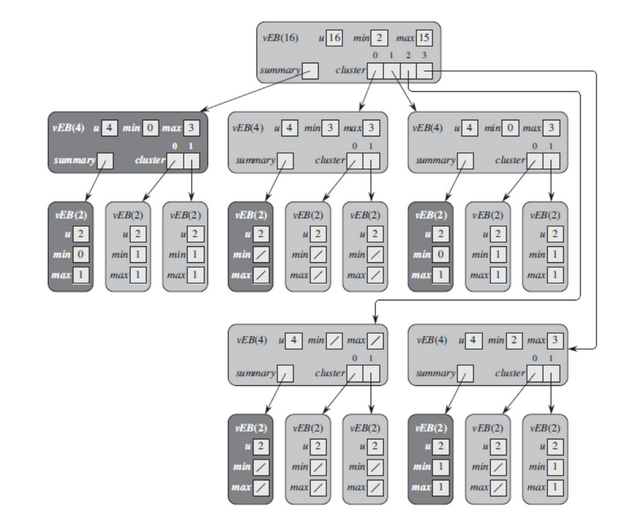
\includegraphics[width=0.72\columnwidth]{vEB.png}
\caption{Van Emde Boas Tree}
\label{fig:vb}
\end{figure}


\subsubsection{The following operations of vEB Tree are used for the project:}
\begin{enumerate}
\item Insert: insert a m-bit value into the tree. Time Complexity: O(loglogM)
\item Delete: insert a m-bit value into the tree. Time Complexity: O(loglogM)
\item Min/Max: find the minimum/maximum value present in the tree. Time Complexity: O(1)
\end{enumerate}

\section{Kruskal Implementation}
\subsection{Using merge sort}
Steps:
\begin{enumerate}
\item Initialize an empty set A
\item Create V trees, one containing each vertex
\item Sort the edges of the graph G(V,E) in non-descending order by weight
\item For each edge taken in non-descending order by weight, check whether the end points of the edge u, v belong to the same tree. If yes, the edge is discarded, else merge the 2 vertices into a single set and add the edge to A
\end{enumerate}
Time Complexity: O(E LogE)

\subsection{Using Fibonacci Heap}
In this, we use store the edges of the graph in a Fibonacci Heap. We call extract-min each time to get the edge with the smallest weight instead of sorting compared to the standard implementation. Rest of the algorithm remains the same.

Time Complexity: O(E log E)

\subsection{Using vEB Tree}
Used a hash table to store the multiple values of the same key. Once the count of the key goes down to zero, we delete the current min from the tree and update the min.

\section{Implementation Challenges}
\begin{enumerate}
\item In vEB tree, the standard implementation doesn't work when there are duplicate values present in the tree. For this, we had to use a hash table externally to store the edge count of each weight.
\item While comparing vEB, Fibonnaci Heap and merge sort. From complexity it seems, that vEB tree(O(loglogu)) should perform better than Merge sort(O(nlogn)), but in actual, it is the opposite. After deep diving, we realised that the constants for vEB tree are much much higher than others, hence overall vEB tree doesn't perform so well for Kruskal implementation

\end{enumerate}
\section{Results}
\begin{enumerate}
\item Standard Kruskal with merge sort(dsu) outperforms the rest as its constants are much smaller
\item vEB Tree(veb) performs worst at the beginning(less number of edges), but as the edge count increases vEB outperforms Fibonnaci(fib). This is because loglogu has a drastic effect only when u is very high, else logu and loglogu are almost same. Also, the constants for vEB tree are higher than that of Fibonnaci Heap.
\item Tests were done when edges were inserted in random order, increasing order, and decreasing order. In all the 3 cases, the relative performance is consistent.
\item For plotting the data, about 160 data points were used

\end{enumerate}


\section{Time Analysis}

\begin{table}[h!]
  \begin{center}
    \label{tab:table1}
    \begin{tabular}{l|c|r} % <-- Alignments: 1st column left, 2nd middle and 3rd right, with vertical lines in between
      \textbf{Merge Sort} & \textbf{Fibonnaci Heap} & \textbf{Van Emde Boas Tree}\\
      \hline
      O(c1 * ElogE) & O(c2 * ElogE) & O(c3 * Eloglogu)\\
    \end{tabular}
    \caption{Time Complexity Comparison}
  \end{center}
  \footnote{\textit{E is the number of edges}}
\end{table}

\begin{figure}[h!]
\centering
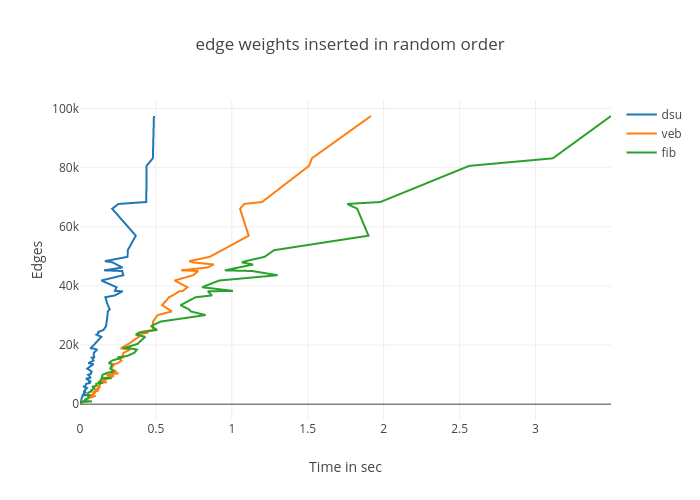
\includegraphics[width=1\columnwidth]{random_data.png}
\caption{Comparison with random edge weights}
\label{fig:vb}
\end{figure}

\begin{figure}[h!]
\centering
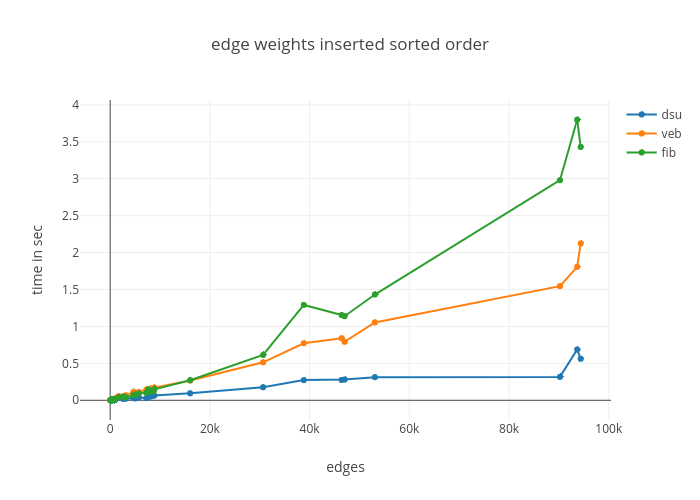
\includegraphics[width=0.8\columnwidth]{sorted_data.png}
\caption{Comparison with sorted edge weights}
\label{fig:vb}
\end{figure}

\begin{figure}[h!]
\centering
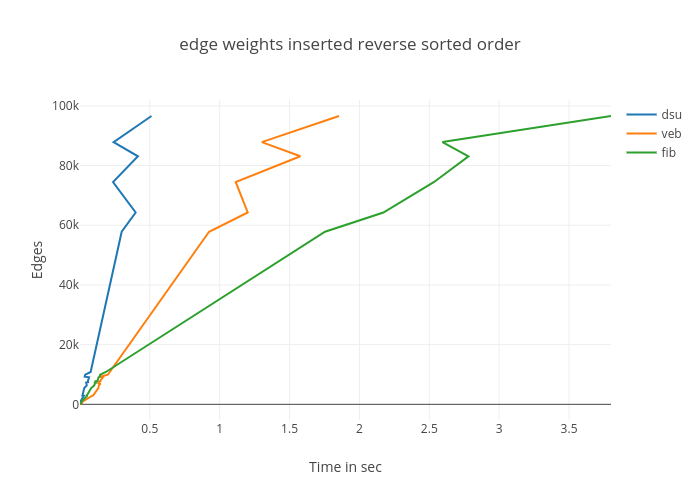
\includegraphics[width=0.8\columnwidth]{rsorted_data.png}
\caption{Comparison with reverse sorted edge weights}
\label{fig:vb}
\end{figure}

\section{End user documentation}
\subsection{Run kruskal algorithm using normal DSU}
    \begin{enumerate}
        \item Enter the directory
        \item Run ./generate to generate 150 files containing random          number of edges with corressponding random edges              weights of range 0-1000, 0-10000, 0-100000
        \item Run ./krudsu.sh to run the python code on each file and         the output for each file will be generated in dsu.txt         with number of edges on which it was run, number of seconds required to compute the mst-cost,          and the mst-cost
\end{enumerate}

\subsection{Run kruskal algorithm using vEB tree}
    \begin{enumerate}
        \item Enter the directory
        \item Run ./generate to generate 150 files containing random          number of edges with corressponding random edges              weights of range 0-1000, 0-10000, 0-100000
        \item Run ./kruveb.sh to run the python code on each file and         the output for each file will be generated in veb.txt         with number of edges on which it was run, number of seconds required to compute the mst-cost,          and the mst-cost
\end{enumerate}
 \subsection{Run kruskal algorithm using fibonacci heap}
    \begin{enumerate}
        \item Enter the directory
        \item Run ./generate to generate 150 files containing random          number of edges with corressponding random edges              weights of range 0-1000, 0-10000, 0-100000
        \item Run ./krufib.sh to run the python code on each file and         the output for each file will be generated in fib.txt         with number of edges on which it was run, number of seconds required to compute the mst-cost,          and the mst-cost
\end{enumerate}   
\subsection{Comparison of time complexity for each implementation}
\begin{enumerate}
        \item Enter the directory
        \item Run ./generate to generate 150 files containing random          number of edges with corressponding random edges              weights of range 0-1000, 0-10000, 0-100000
        \item Run ./setup.sh to generate plot that shows the comparison of time required to output mst-cost for each of the implementation 
\end{enumerate}
\subsection{Running the code on custom user input}
    \subsubsection{Running vEB tree implementation}
    \begin{enumerate}
        \item Run the python code using python3 kruskl\_veb.py
        \item Enter number of edges
        \item Enter the number of vertices
        \item For each edge
        \begin{enumerate}
        \item Enter linked vertex 1
        \item Enter linked vertex 2
        \item Enter the edge weight
        \end{enumerate}
        \item Enter to get the number of input edges on which it was run, time required to get mst-cost and their corresponding mst-cost
    \end{enumerate}
    \subsubsection{Running normal DSU tree implementation}
    \begin{enumerate}
        \item Run the python code using python3 krudsu.py
        \item Enter number of edges
        \item Enter the number of vertices
        \item For each edge
        \begin{enumerate}
        \item Enter linked vertex 1
        \item Enter linked vertex 2
        \item Enter the edge weight
        \end{enumerate}
        \item Enter to get the number of input edges on which it was run, time required to get mst-cost and their corresponding mst-cost
    \end{enumerate}
    \subsubsection{Running fibonacci tree implementation}
    \begin{enumerate}
        \item Run the python code using python3 krskal\_fibbonacci.py
        \item Enter number of edges
        \item Enter the number of vertices
         \item For each edge
        \begin{enumerate}
        \item Enter linked vertex 1
        \item Enter linked vertex 2
        \item Enter the edge weight
        \end{enumerate}
        \item Enter to get the number of input edges on which it was run, time required to get mst-cost and their corresponding mst-cost
    \end{enumerate}
\section{References}
\begin{enumerate}
    \item\href{https://www.cl.cam.ac.uk/teaching/1314/AlgorithII/2013-stajano-algs2-students-handout.pdf}{Algorithm's II university of cambridge}
    \item\href{https://ocw.mit.edu/courses/electrical-engineering-and-computer-science/6-046j-design-and-analysis-of-algorithms-spring-2015/lecture-notes/MIT6_046JS15_lec04.pdf}{Lecture 4: Divide and Conquer:van Emde Boas Trees}
    \item\href{https://mcdtu.files.wordpress.com/2017/03/introduction-to-algorithms-3rd-edition-sep-2010.pdf}{Introduction to Algorithms by CLRS}
    \item\href{https://ocw.mit.edu/courses/electrical-engineering-and-computer-science/6-854j-advanced-algorithms-fall-2008/lecture-notes/lec1.pdf}{Fibonacci Heaps by MIT}
    \item\href{http://web.stanford.edu/class/archive/cs/cs166/cs166.1146/lectures/07/Small07.pdf}{Fibonacci Heaps by Stanford}
    \item\href{http://www.cse.iitd.ernet.in/~naveen/courses/CSL630/x02-fiboheap.pdf}{Fibonacci Heaps by IIT Delhi}
    \item\href{https://ocw.mit.edu/courses/electrical-engineering-and-computer-science/6-046j-design-and-analysis-of-algorithms-spring-2012/lecture-notes/MIT6_046JS12_lec04.pdf}{Kruskal's Algorithm using disjint set union find algorithm}
    \item\href{https://en.wikipedia.org/wiki/Disjoint-set_data_structure}{Disjint set data structure}
    \item\href{https://en.wikipedia.org/wiki/Fibonacci_heap}{Fibbonaci Heap}
    \item\href{https://en.wikipedia.org/wiki/Van_Emde_Boas_tree}{Van Emde Boas Tree}
\end{enumerate}
\end{document}
